\documentclass{beamer}

\usepackage[utf8]{inputenc}
\usepackage{enumitem}
\usetheme{Madrid}
\usecolortheme{default}
\usepackage{amsmath,amssymb,amsfonts,amsthm}
\usepackage{txfonts}
\usepackage{tikz}
\usepackage{graphicx}
\usepackage{minted}
\usepackage{gvv}
\usepackage{gvv-book}
\setbeamertemplate{page number in head/foot}[totalframenumber]

\title{1.4.20: Section Formula Problem}
\author{Aditya Mishra - ee25btech11005}
\date{August 27, 2025}

\begin{document}

\frame{\titlepage}

\begin{frame}{Question}
Find the coordinates of the point which divides the line segment joining
\[
A(-2,3,5), \quad B(1,-4,6)
\]
in the ratio
\begin{enumerate}[label=(\alph*)]
    \item \(2 : 3\) internally
    \item \(2 : 3\) externally
\end{enumerate}
\end{frame}

\begin{frame}{Given Information}
Given vector \(\mathbf{A}\):
\[
\begin{bmatrix} -2 \\ 3 \\ 5 \end{bmatrix}
\]
Given vector \(\mathbf{B}\):
\[
\begin{bmatrix} 1 \\ -4 \\ 6 \end{bmatrix}
\]
\end{frame}

\begin{frame}{Required Formulae}
Internal division:
\[
P = \frac{m \mathbf{B} + n \mathbf{A}}{m + n}
\]

External division:
\[
Q = \frac{m \mathbf{B} - n \mathbf{A}}{m - n}
\]
\end{frame}

\begin{frame}{Solution - Internal}
\[
P = \frac{2 \begin{bmatrix} 1 \\ -4 \\ 6 \end{bmatrix} + 3 \begin{bmatrix} -2 \\ 3 \\ 5 \end{bmatrix}}{5}
= \frac{\begin{bmatrix} 2 - 6 \\ -8 + 9 \\ 12 + 15 \end{bmatrix}}{5}
= \begin{bmatrix} -\frac{4}{5} \\ \frac{1}{5} \\ \frac{27}{5} \end{bmatrix}
\]
\end{frame}

\begin{frame}{Solution - External}
\[
Q = \frac{2 \begin{bmatrix} 1 \\ -4 \\ 6 \end{bmatrix} - 3 \begin{bmatrix} -2 \\ 3 \\ 5 \end{bmatrix}}{2 - 3}
= \frac{\begin{bmatrix} 2 + 6 \\ -8 - 9 \\ 12 - 15 \end{bmatrix}}{-1}
= \begin{bmatrix} -8 \\ 17 \\ 3 \end{bmatrix}
\]
\end{frame}

\begin{frame}[fragile]{Python Code-Plot}
\begin{minted}[fontsize=\footnotesize]{python}
import matplotlib.pyplot as plt
from mpl_toolkits.mplot3d import Axes3D

A = (-2, 3, 5)
B = (1, -4, 6)

P = (
    (2*B[0] + 3*A[0]) / 5,
    (2*B[1] + 3*A[1]) / 5,
    (2*B[2] + 3*A[2]) / 5
)

Q = (
    (2*B[0] - 3*A[0]) / (2-3),
    (2*B[1] - 3*A[1]) / (2-3),
    (2*B[2] - 3*A[2]) / (2-3)
)

print("Internal Division Point:", P)
print("External Division Point:", Q)
\end{minted}
\end{frame}

\begin{frame}[fragile]{Python Code-Plot}
\begin{minted}[fontsize=\footnotesize]{python}
fig = plt.figure(figsize=(8,8))
ax = fig.add_subplot(111, projection='3d')

ax.plot([A[0], B[0]], [A[1], B[1]], [A[2], B[2]], color='blue')

def plot_point(pt, label, color):
    ax.scatter(*pt, color=color, s=60)
    ax.text(pt[0], pt[1], pt[2], f"{label}{pt}", fontsize=10)

plot_point(A, "A", "red")
plot_point(B, "B", "red")
plot_point(P, "P", "green")
plot_point(Q, "Q", "purple")

ax.set_xlabel('X-axis')
ax.set_ylabel('Y-axis')
ax.set_zlabel('Z-axis')
ax.set_title('3D Division of Line Segment')


\end{minted}
\end{frame}

\begin{frame}[fragile]{Python Code-Plot}
\begin{minted}[fontsize=\footnotesize]{python}
ax.set_xlim(-10, 5)
ax.set_ylim(-10, 20)
ax.set_zlim(0, 10)

plt.savefig("Figs/graph.png")
plt.show()
\end{minted}
\end{frame}


\begin{frame}[fragile]{Python ctypes Call}
\begin{minted}[fontsize=\footnotesize]{python}
import ctypes

lib = ctypes.CDLL('./mat1.so')

lib.sectionFormula.argtypes = [
    ctypes.POINTER(ctypes.c_float),
    ctypes.POINTER(ctypes.c_float),
    ctypes.c_float,
    ctypes.c_float,
    ctypes.POINTER(ctypes.c_float)
]
\end{minted}
\end{frame}

\begin{frame}[fragile]{Python ctypes Call}
\begin{minted}[fontsize=\footnotesize]{python}
lib.sectionFormula.restype = None

lib.sectionFormulaExternal.argtypes = [
    ctypes.POINTER(ctypes.c_float),
    ctypes.POINTER(ctypes.c_float),
    ctypes.c_float,
    ctypes.c_float,
    ctypes.POINTER(ctypes.c_float)
]

lib.sectionFormulaExternal.restype = None

p1 = (ctypes.c_float * 3)(-2.0, 3.0, 5.0)
p2 = (ctypes.c_float * 3)(1.0, -4.0, 6.0)

res_internal = (ctypes.c_float * 3)()
res_external = (ctypes.c_float * 3)()

m = 2.0
n = 3.0
\end{minted}
\end{frame}

\begin{frame}[fragile]{Python ctypes Call}
\begin{minted}[fontsize=\footnotesize]{python}
lib.sectionFormula(p1, p2, m, n, res_internal)
lib.sectionFormulaExternal(p1, p2, m, n, res_external)

print("Internal division (2:3): [{:.2f}, {:.2f}, {:.2f}]".format(
    res_internal[0], res_internal[1], res_internal[2]
))

print("External division (2:3): [{:.2f}, {:.2f}, {:.2f}]".format(
    res_external[0], res_external[1], res_external[2]
))
\end{minted}
\end{frame}
\begin{frame}[fragile]{C Code}
\begin{minted}[fontsize=\footnotesize]{c}
void sectionFormula(float p1[3], float p2[3], float m, float n,
float res[3]) {
    res[0] = (m * p2[0] + n * p1[0]) / (m + n);
    res[1] = (m * p2[1] + n * p1[1]) / (m + n);
    res[2] = (m * p2[2] + n * p1[2]) / (m + n);
}

void sectionFormulaExternal(float p1[3], float p2[3], float m, 
float n, float res[3]) {
    res[0] = (m * p2[0] - n * p1[0]) / (m - n);
    res[1] = (m * p2[1] - n * p1[1]) / (m - n);
    res[2] = (m * p2[2] - n * p1[2]) / (m - n);
}
\end{minted}
\end{frame}

\begin{frame}{Plot}
\begin{figure}
\centering
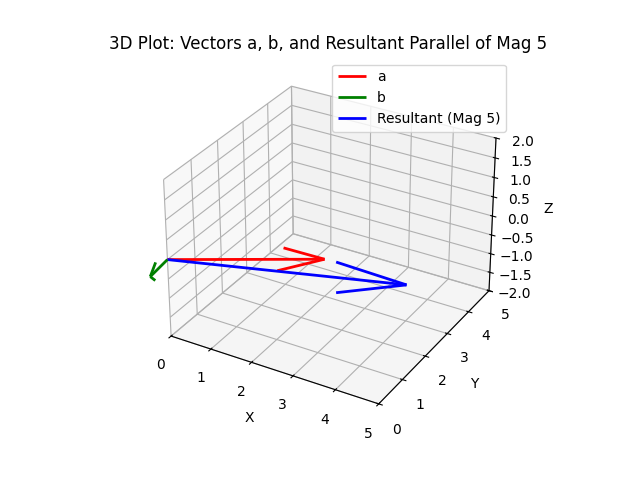
\includegraphics[width=0.8\linewidth]{Figs/graph.png}
\caption{3D Plot of points \(A, B, P, Q\)}
\label{fig:graph}
\end{figure}
\end{frame}
\end{document}
